\documentclass[preprint, 3p,
authoryear]{elsarticle} %review=doublespace preprint=single 5p=2 column
%%% Begin My package additions %%%%%%%%%%%%%%%%%%%

\usepackage[hyphens]{url}

  \journal{DATA 698} % Sets Journal name

\usepackage{lineno} % add

\usepackage{graphicx}
%%%%%%%%%%%%%%%% end my additions to header

\usepackage[T1]{fontenc}
\usepackage{lmodern}
\usepackage{amssymb,amsmath}
\usepackage{ifxetex,ifluatex}
\usepackage{fixltx2e} % provides \textsubscript
% use upquote if available, for straight quotes in verbatim environments
\IfFileExists{upquote.sty}{\usepackage{upquote}}{}
\ifnum 0\ifxetex 1\fi\ifluatex 1\fi=0 % if pdftex
  \usepackage[utf8]{inputenc}
\else % if luatex or xelatex
  \usepackage{fontspec}
  \ifxetex
    \usepackage{xltxtra,xunicode}
  \fi
  \defaultfontfeatures{Mapping=tex-text,Scale=MatchLowercase}
  \newcommand{\euro}{€}
\fi
% use microtype if available
\IfFileExists{microtype.sty}{\usepackage{microtype}}{}
\usepackage[]{natbib}
\bibliographystyle{plainnat}

\usepackage{graphicx}
\ifxetex
  \usepackage[setpagesize=false, % page size defined by xetex
              unicode=false, % unicode breaks when used with xetex
              xetex]{hyperref}
\else
  \usepackage[unicode=true]{hyperref}
\fi
\hypersetup{breaklinks=true,
            bookmarks=true,
            pdfauthor={},
            pdftitle={Adverse Drug Events in New York Hospitals: Prediction and Associated Costs},
            colorlinks=false,
            urlcolor=blue,
            linkcolor=magenta,
            pdfborder={0 0 0}}

\setcounter{secnumdepth}{5}
% Pandoc toggle for numbering sections (defaults to be off)

% Pandoc syntax highlighting
\usepackage{color}
\usepackage{fancyvrb}
\newcommand{\VerbBar}{|}
\newcommand{\VERB}{\Verb[commandchars=\\\{\}]}
\DefineVerbatimEnvironment{Highlighting}{Verbatim}{commandchars=\\\{\}}
% Add ',fontsize=\small' for more characters per line
\usepackage{framed}
\definecolor{shadecolor}{RGB}{248,248,248}
\newenvironment{Shaded}{\begin{snugshade}}{\end{snugshade}}
\newcommand{\AlertTok}[1]{\textcolor[rgb]{0.94,0.16,0.16}{#1}}
\newcommand{\AnnotationTok}[1]{\textcolor[rgb]{0.56,0.35,0.01}{\textbf{\textit{#1}}}}
\newcommand{\AttributeTok}[1]{\textcolor[rgb]{0.77,0.63,0.00}{#1}}
\newcommand{\BaseNTok}[1]{\textcolor[rgb]{0.00,0.00,0.81}{#1}}
\newcommand{\BuiltInTok}[1]{#1}
\newcommand{\CharTok}[1]{\textcolor[rgb]{0.31,0.60,0.02}{#1}}
\newcommand{\CommentTok}[1]{\textcolor[rgb]{0.56,0.35,0.01}{\textit{#1}}}
\newcommand{\CommentVarTok}[1]{\textcolor[rgb]{0.56,0.35,0.01}{\textbf{\textit{#1}}}}
\newcommand{\ConstantTok}[1]{\textcolor[rgb]{0.00,0.00,0.00}{#1}}
\newcommand{\ControlFlowTok}[1]{\textcolor[rgb]{0.13,0.29,0.53}{\textbf{#1}}}
\newcommand{\DataTypeTok}[1]{\textcolor[rgb]{0.13,0.29,0.53}{#1}}
\newcommand{\DecValTok}[1]{\textcolor[rgb]{0.00,0.00,0.81}{#1}}
\newcommand{\DocumentationTok}[1]{\textcolor[rgb]{0.56,0.35,0.01}{\textbf{\textit{#1}}}}
\newcommand{\ErrorTok}[1]{\textcolor[rgb]{0.64,0.00,0.00}{\textbf{#1}}}
\newcommand{\ExtensionTok}[1]{#1}
\newcommand{\FloatTok}[1]{\textcolor[rgb]{0.00,0.00,0.81}{#1}}
\newcommand{\FunctionTok}[1]{\textcolor[rgb]{0.00,0.00,0.00}{#1}}
\newcommand{\ImportTok}[1]{#1}
\newcommand{\InformationTok}[1]{\textcolor[rgb]{0.56,0.35,0.01}{\textbf{\textit{#1}}}}
\newcommand{\KeywordTok}[1]{\textcolor[rgb]{0.13,0.29,0.53}{\textbf{#1}}}
\newcommand{\NormalTok}[1]{#1}
\newcommand{\OperatorTok}[1]{\textcolor[rgb]{0.81,0.36,0.00}{\textbf{#1}}}
\newcommand{\OtherTok}[1]{\textcolor[rgb]{0.56,0.35,0.01}{#1}}
\newcommand{\PreprocessorTok}[1]{\textcolor[rgb]{0.56,0.35,0.01}{\textit{#1}}}
\newcommand{\RegionMarkerTok}[1]{#1}
\newcommand{\SpecialCharTok}[1]{\textcolor[rgb]{0.00,0.00,0.00}{#1}}
\newcommand{\SpecialStringTok}[1]{\textcolor[rgb]{0.31,0.60,0.02}{#1}}
\newcommand{\StringTok}[1]{\textcolor[rgb]{0.31,0.60,0.02}{#1}}
\newcommand{\VariableTok}[1]{\textcolor[rgb]{0.00,0.00,0.00}{#1}}
\newcommand{\VerbatimStringTok}[1]{\textcolor[rgb]{0.31,0.60,0.02}{#1}}
\newcommand{\WarningTok}[1]{\textcolor[rgb]{0.56,0.35,0.01}{\textbf{\textit{#1}}}}

% tightlist command for lists without linebreak
\providecommand{\tightlist}{%
  \setlength{\itemsep}{0pt}\setlength{\parskip}{0pt}}



\usepackage{amsmath}
\usepackage{booktabs}
\usepackage{caption}
\usepackage{longtable}



\begin{document}


\begin{frontmatter}

  \title{Adverse Drug Events in New York Hospitals: Prediction and
Associated Costs}
    \author[CUNY School of Profesional Services]{Thomas Hill%
  \corref{cor1}%
  \fnref{1}}
   \ead{thomas.hill82@spsmail.cuny.edu} 
      \cortext[cor1]{Corresponding author}
  
  \begin{abstract}
  
  \end{abstract}
    \begin{keyword}
    Data Science \sep 
    Adverse Drug Event
  \end{keyword}
  
 \end{frontmatter}

\hypertarget{abstract}{%
\subsection{Abstract}\label{abstract}}

Adverse drug events are a serious consequence of medication therapy.
Previous research has associated adverse events with poorer outcomes,
and suggested some patients are at higher risks for side effects. Using
hospital admission records from New York State in 2018, the most common
adverse events were obtained and the overall impact of an adverse drug
event was estimated. A model for predicting prospective risk based on
patient characteristics was developed.

\hypertarget{background}{%
\subsection{Background}\label{background}}

Adverse drug event (ADE) is the comprehensive term for the negative
effects related to medication therapy. ADE's may be unforeseen or known,
and vary in severity from untoward changes in laboratory values to
injury and death. Some medications have therapeutic dosing close to
their corresponding toxic dose, which is a characteristic described as
narrow therapeutic index. In these situations, prospective monitoring
may be warranted.

In the United States, the Food and Drug Administration manages the
publicly available FDA Adverse Event Reporting System to collect
voluntary reports from consumers and healthcare practitioners. In
contrast, New York State mandates that adverse events occurring in
hospitals and diagnostic centers are reported.

The US government also has a program offering access to detailed
hospital admissions data through its Agency for Healthcare Research and
Quality (AHRQ). It combines hospital and admission characteristics as
well as information about charges. The research done using these data is
extensive, including applications to monitoring ADE's.

\hypertarget{dataset}{%
\subsection{Dataset}\label{dataset}}

The dataset is available through AHRQ's healthcare cost and utilization
project (HCUP), which offers several options for obtaining admissions
information. There are annual reports spanning the entire United States,
as well as more detailed reports for each state. Datasets for each year
are further broken down into pediatric and adult, as well as inpatient,
emergency, ambulatory, and readmissions data. The most recent dataset
available at the time is 2018, and while the variables reported are
mostly uniform there are additional admission characteristics that are
reported in some states.

Data are available in two separate files: CORE and CHARGE files. The
CORE file represents patient characteristics, timing of admission and
length of stay; it also includes diagnoses and procedures as described
by the International Classification of Diseases (ICD-10) as well as
diagnosis-related groups (DRG's) used extensively by Medicare. The
CHARGE file contains dollar and unit amounts of services rendered during
each individual admission. There is also a Healthcare Common Procedure
Coding System (HCPCS) revenue code as an additional descriptor of the
hospital cost center where the charge originated. Each observation in
both files has a unique admission number designated by the KEY
attribute. In total, there were \#\#\# unique admissions with over
\#\#\# charges in 2018.

These data are also available for free via HCUPnet, a data query tool
accessible on the AHRQ website. No API is available for repeated or
programmable querying. HCUPnet returns counts and rates for selected
diagnoses by year and region, but remains useful to researchers to
confirm the validity of their own findings.

\hypertarget{methods}{%
\subsection{Methods}\label{methods}}

The two main files were first loaded into SPSS to be translated using
HCUP's provided loader program. These were then converted to .csv format
and loaded into a local SQL database. The CORE file for New York state
has \#\#\# features, many of which are used to hold ICD codes and dates
for ICD procedure codes. The ICD has three generic codes used for ADE's,
seen in Table \#\#\#. Based on previous research, there are also \#\#\#
additional codes located in described in other ICD categories that are
also correlated with the absence of an event. The strength of
associations is described in Table \#\#\#. Admissions were determined by
filtering ICD codes where an ADE was likely present.

There \#\#\# additional databases I used for labeling purposes. I used a
.csv with all available ICD diagnosis codes and subcodes to interpret
diagnoses. There was also a corresponding list of all ICD procedure
codes. A ny.gov list of FIPS codes was used to translate patient
location into county and then region information. Finally, for the
CHARGES file, I reformatted a table available on New York's Department
of Health website for descriptions of each revenue code.

\hypertarget{data-wrangling}{%
\subsubsection{Data Wrangling}\label{data-wrangling}}

The dataset required extensive transformation to better visualize and
explore each feature. ICD diagnosis codes are located in 35 columns,
with an additional 35 columns indicating whether the diagnosis was
present upon admission. Similarly, each ICD procedure code filled one of
25 columns, plus 50 additional columns specifying the date and year. The
columns containing the codes were converted to one-hot encoded columns
for the most common diagnoses. Diagnoses were sometimes specific,
e.g.~`G40' for epileptic seizure, or more general by searching for all
codes starting with `G' indicating diseases of the nervous system.
Procedures were handled identically, with the added step that multiple
identical procedures were counted more than once. For example, if the
patient received three infusions of platelets, the value would be `3'
rather than `1'.

\hypertarget{missing-values}{%
\paragraph{Missing Values}\label{missing-values}}

For blood pressure and heart rate, values were available for a minority
of observations. Instead of ignoring these data, each was refactored
according to clinical categories, like Stage I Hypertension or
bradycardia. In the case that patient location was unavailable via FIPS
code, the hospital NPI was used as an approximate location by manually
replacing with the local code.

\begin{verbatim}
## Warning in recode.numeric(.x, !!!values, .default = .default, .missing
## = .missing): NAs introduced by coercion

## Warning in recode.numeric(.x, !!!values, .default = .default, .missing
## = .missing): NAs introduced by coercion
\end{verbatim}

\begin{Shaded}
\begin{Highlighting}[]
\DocumentationTok{\#\#{-}Average LOS }


\NormalTok{ade\_cost }\OtherTok{\textless{}{-}}\NormalTok{ ade\_flag }\SpecialCharTok{\%\textgreater{}\%} \FunctionTok{select}\NormalTok{(has\_ade, LOS\_X, TOTCHG\_X) }
\NormalTok{ade\_cost}\SpecialCharTok{$}\NormalTok{LOS\_X[ade\_cost}\SpecialCharTok{$}\NormalTok{LOS\_X }\SpecialCharTok{==} \DecValTok{0}\NormalTok{] }\OtherTok{\textless{}{-}} \DecValTok{1} \CommentTok{\#change \textquotesingle{}zero\textquotesingle{} length of stay to \textquotesingle{}1\textquotesingle{}}

\NormalTok{ade\_cost }\SpecialCharTok{\%\textgreater{}\%}
    \FunctionTok{summarize}\NormalTok{(}\AttributeTok{AVG\_LOS =} \FunctionTok{mean}\NormalTok{(LOS\_X, }\AttributeTok{na.rm =} \ConstantTok{TRUE}\NormalTok{))}

\NormalTok{ade\_cost }\SpecialCharTok{\%\textgreater{}\%}
  \FunctionTok{filter}\NormalTok{(has\_ade }\SpecialCharTok{==}\DecValTok{1}\NormalTok{) }\SpecialCharTok{\%\textgreater{}\%}
    \FunctionTok{summarize}\NormalTok{(}\AttributeTok{AVG\_LOS =} \FunctionTok{mean}\NormalTok{(LOS\_X, }\AttributeTok{na.rm =} \ConstantTok{TRUE}\NormalTok{))}

\NormalTok{ade\_cost }\SpecialCharTok{\%\textgreater{}\%}
    \FunctionTok{summarize}\NormalTok{(}\AttributeTok{med\_los =} \FunctionTok{median}\NormalTok{(LOS\_X, }\AttributeTok{na.rm =} \ConstantTok{TRUE}\NormalTok{))}

\NormalTok{ade\_cost }\SpecialCharTok{\%\textgreater{}\%}
  \FunctionTok{filter}\NormalTok{(has\_ade }\SpecialCharTok{==}\DecValTok{1}\NormalTok{) }\SpecialCharTok{\%\textgreater{}\%}
\FunctionTok{summarize}\NormalTok{(}\AttributeTok{med\_los =} \FunctionTok{median}\NormalTok{(LOS\_X, }\AttributeTok{na.rm =} \ConstantTok{TRUE}\NormalTok{))}
\end{Highlighting}
\end{Shaded}

\begin{verbatim}
##   avg_charge
## 1   56839.97
\end{verbatim}

\begin{verbatim}
##   avg_charge
## 1     104979
\end{verbatim}

\begin{verbatim}
##   avg_charge
## 1   32149.41
\end{verbatim}

\begin{verbatim}
##   avg_charge
## 1   51858.46
\end{verbatim}

\begin{Shaded}
\begin{Highlighting}[]
\NormalTok{stats\_table }\OtherTok{\textless{}{-}} \FunctionTok{read.csv}\NormalTok{(}\StringTok{\textquotesingle{}descriptive\_statistics.csv\textquotesingle{}}\NormalTok{)}
\FunctionTok{colnames}\NormalTok{(stats\_table) }\OtherTok{\textless{}{-}} \FunctionTok{c}\NormalTok{(}\StringTok{\textquotesingle{}Characteristics\textquotesingle{}}\NormalTok{, }\StringTok{\textquotesingle{}Total Population\textquotesingle{}}\NormalTok{, }\StringTok{\textquotesingle{}Target Population\textquotesingle{}}\NormalTok{)}

\NormalTok{stats\_table[}\DecValTok{1}\NormalTok{,}\DecValTok{2}\NormalTok{] }\OtherTok{\textless{}{-}} \FunctionTok{prettyNum}\NormalTok{(}\AttributeTok{big.mark =} \StringTok{\textquotesingle{},\textquotesingle{}}\NormalTok{,stats\_table[}\DecValTok{1}\NormalTok{,}\DecValTok{2}\NormalTok{]) }
\NormalTok{stats\_table[}\DecValTok{1}\NormalTok{,}\DecValTok{3}\NormalTok{] }\OtherTok{\textless{}{-}} \FunctionTok{prettyNum}\NormalTok{(}\AttributeTok{big.mark =} \StringTok{\textquotesingle{},\textquotesingle{}}\NormalTok{,stats\_table[}\DecValTok{1}\NormalTok{,}\DecValTok{3}\NormalTok{]) }

\NormalTok{stats\_table }\SpecialCharTok{\%\textgreater{}\%}
\FunctionTok{replace}\NormalTok{(}\FunctionTok{is.na}\NormalTok{(.), }\StringTok{\textquotesingle{} \textquotesingle{}}\NormalTok{) }\SpecialCharTok{\%\textgreater{}\%}
   \FunctionTok{gt}\NormalTok{() }\SpecialCharTok{\%\textgreater{}\%}
  \FunctionTok{tab\_header}\NormalTok{(}\StringTok{"2018 New York Hospital Admissions, Baseline Characteristics"}\NormalTok{)}
\end{Highlighting}
\end{Shaded}

\captionsetup[table]{labelformat=empty,skip=1pt}
\begin{longtable}{lll}
\caption*{
{\large 2018 New York Hospital Admissions, Baseline Characteristics}
} \\ 
\toprule
Characteristics & Total Population & Target Population \\ 
\midrule
n & 2,018,259 & 42,829 \\ 
Age (years & 58.3 & 62.2 \\ 
Female (\%) & 56.2 & 48.9 \\ 
Race (\%) &   &   \\ 
White & 54.6 & 59.7 \\ 
Black & 17.1 & 13 \\ 
Hispanic & 13.8 & 13.1 \\ 
AAPI & 4.6 & 4.1 \\ 
Native American & 0.2 & 0.7 \\ 
Other/Missing & 9.7 & 9.7 \\ 
Hispanic (\%) &   &   \\ 
Not Hispanic & 81.6 & 83 \\ 
Hispanic, White & 3.2 & 2.8 \\ 
Hispanic, Black & 0.7 & 0.6 \\ 
Hispanic, Other Race & 9.8 & 9.8 \\ 
Missing & 4.6 & 3.9 \\ 
ED Admission (\%) & 67 & 43.8 \\ 
Died (\%) & 2.4 & 4.8 \\ 
Length of Stay (days) & 5.7 & 9.2 \\ 
Median Length of Stay (days) & 3 & 6 \\ 
Number of Diagnoses & 12.1 & 18 \\ 
Number of Procedures & 2.1 & 2.9 \\ 
Charge (\$1K) & 56.8 & 105 \\ 
Median Charge ( \$1K) & 32.1 & 58.9 \\ 
Charge per Day (\$1K) & 13.4 & 12.1 \\ 
Median Charge per Day (\$1K) & 9.4 & 9.9 \\ 
\bottomrule
\end{longtable}

\begin{Shaded}
\begin{Highlighting}[]
\FunctionTok{ggplot}\NormalTok{(ade\_flag, }\FunctionTok{aes}\NormalTok{(}\AttributeTok{x =}\NormalTok{ TOTCHG\_X, }\AttributeTok{fill =}\NormalTok{ has\_ade)) }\SpecialCharTok{+}
  \FunctionTok{geom\_density}\NormalTok{(}\AttributeTok{alpha =} \FloatTok{0.4}\NormalTok{) }\SpecialCharTok{+}
  \FunctionTok{labs}\NormalTok{(}\AttributeTok{x =} \StringTok{\textquotesingle{}Total Average of Hospital Admission, USD\textquotesingle{}}\NormalTok{, }\AttributeTok{y =} \StringTok{\textquotesingle{}Proportion of Each Population\textquotesingle{}}\NormalTok{, }\AttributeTok{title =} \StringTok{\textquotesingle{}Average Cost Per day of Inpatient Visit\textquotesingle{}}\NormalTok{, }\AttributeTok{fill =} \StringTok{\textquotesingle{}Presence of ADE\textquotesingle{}}\NormalTok{) }\SpecialCharTok{+}
  \FunctionTok{scale\_x\_continuous}\NormalTok{(}\AttributeTok{trans =} \StringTok{\textquotesingle{}log10\textquotesingle{}}\NormalTok{, }\AttributeTok{labels =}\NormalTok{ scales}\SpecialCharTok{::}\FunctionTok{dollar\_format}\NormalTok{()) }\SpecialCharTok{+}
  \FunctionTok{theme}\NormalTok{(}\AttributeTok{legend.position =} \FunctionTok{c}\NormalTok{(}\FloatTok{0.25}\NormalTok{,}\FloatTok{0.75}\NormalTok{))}
\end{Highlighting}
\end{Shaded}

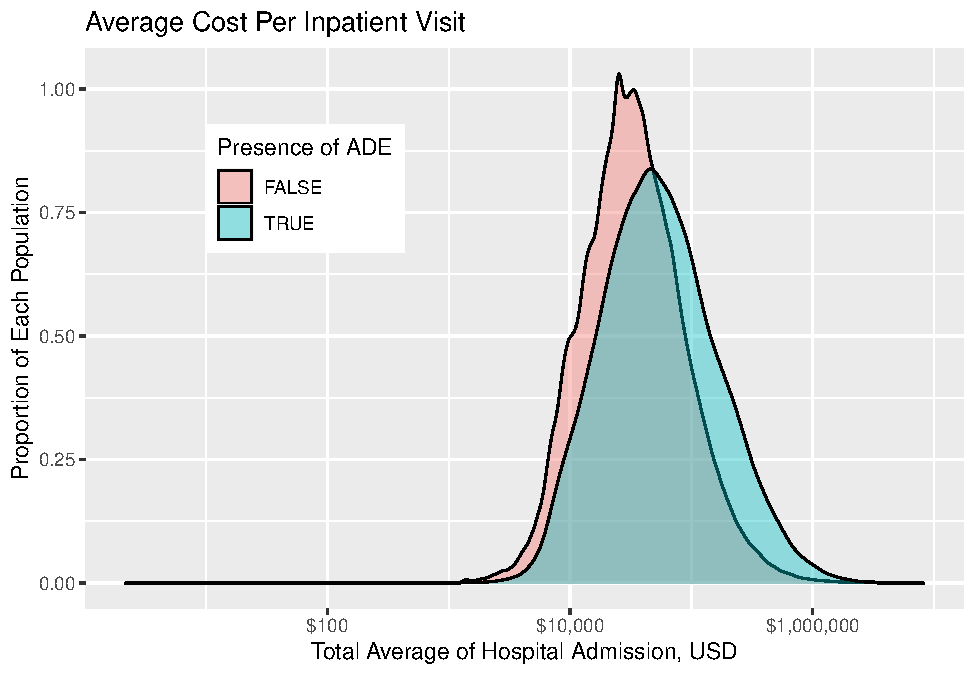
\includegraphics{final-project-paper_files/figure-latex/charge-plot-1.pdf}

\begin{Shaded}
\begin{Highlighting}[]
\FunctionTok{ggplot}\NormalTok{(ade\_cost, }\FunctionTok{aes}\NormalTok{(cost\_per\_day, }\AttributeTok{fill =}\NormalTok{ has\_ade)) }\SpecialCharTok{+}
  \FunctionTok{geom\_density}\NormalTok{(}\AttributeTok{alpha =} \FloatTok{0.4}\NormalTok{) }\SpecialCharTok{+}
  \FunctionTok{scale\_x\_continuous}\NormalTok{(}\AttributeTok{trans =} \StringTok{\textquotesingle{}log10\textquotesingle{}}\NormalTok{, }\AttributeTok{labels =}\NormalTok{ scales}\SpecialCharTok{::}\FunctionTok{dollar\_format}\NormalTok{()) }\SpecialCharTok{+}
  \FunctionTok{labs}\NormalTok{(}\AttributeTok{x =} \StringTok{\textquotesingle{}Average Cost per Day of Hospital Admission, USD\textquotesingle{}}\NormalTok{, }\AttributeTok{y =} \StringTok{\textquotesingle{}Proportion of Each Population\textquotesingle{}}\NormalTok{, }\AttributeTok{title =} \StringTok{\textquotesingle{}Average Cost per day of Inpatient Visit\textquotesingle{}}\NormalTok{, }\AttributeTok{fill =} \StringTok{\textquotesingle{}Presence of ADE\textquotesingle{}}\NormalTok{) }\SpecialCharTok{+}
  \FunctionTok{theme}\NormalTok{(}\AttributeTok{legend.position =} \FunctionTok{c}\NormalTok{(}\FloatTok{0.25}\NormalTok{,}\FloatTok{0.75}\NormalTok{))}
\end{Highlighting}
\end{Shaded}

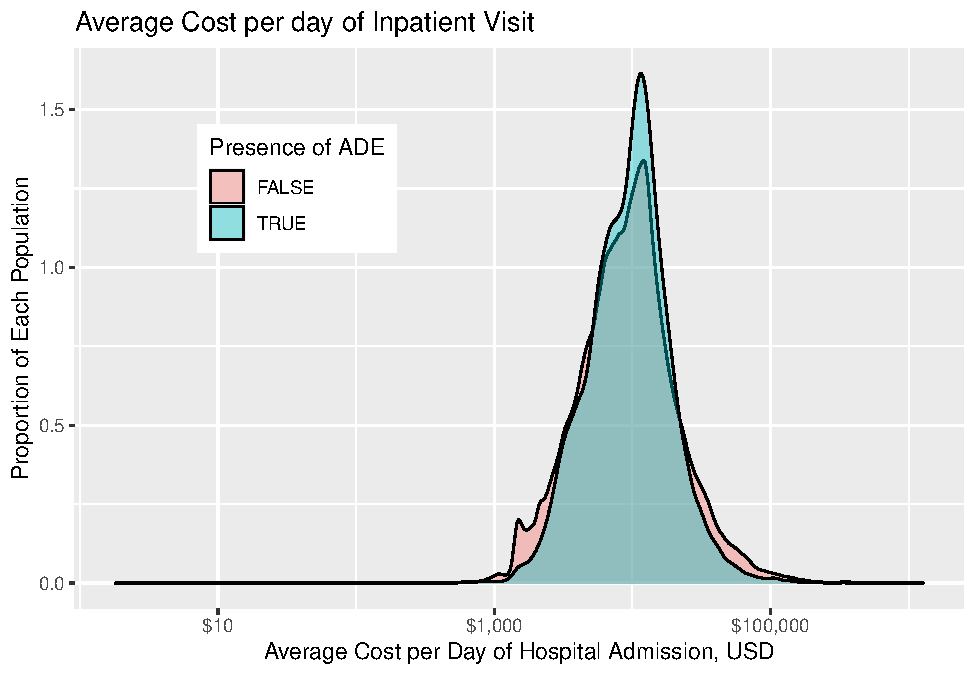
\includegraphics{final-project-paper_files/figure-latex/cost-per-day-plot-1.pdf}

\hypertarget{results}{%
\subsection{Results}\label{results}}

\hypertarget{admitting-diagnosis}{%
\subsubsection{Admitting Diagnosis}\label{admitting-diagnosis}}

\begin{Shaded}
\begin{Highlighting}[]
\NormalTok{ade\_admitting }\OtherTok{\textless{}{-}}\NormalTok{ ade\_flag }\SpecialCharTok{\%\textgreater{}\%} \CommentTok{\#most common ADEs, admitting only}
\NormalTok{  dplyr}\SpecialCharTok{::}\FunctionTok{select}\NormalTok{(I10\_DX\_Admitting) }\SpecialCharTok{\%\textgreater{}\%}
  \FunctionTok{group\_by}\NormalTok{(I10\_DX\_Admitting) }\SpecialCharTok{\%\textgreater{}\%}
  \FunctionTok{summarize}\NormalTok{(}\AttributeTok{n\_patients =} \FunctionTok{n}\NormalTok{()) }\SpecialCharTok{\%\textgreater{}\%}
  \FunctionTok{arrange}\NormalTok{(}\FunctionTok{desc}\NormalTok{(n\_patients)) }\SpecialCharTok{\%\textgreater{}\%}
  \FunctionTok{head}\NormalTok{(}\DecValTok{10}\NormalTok{) }\SpecialCharTok{\%\textgreater{}\%}
  \FunctionTok{left\_join}\NormalTok{(icd, }\FunctionTok{c}\NormalTok{(}\StringTok{\textquotesingle{}I10\_DX\_Admitting\textquotesingle{}} \OtherTok{=} \StringTok{\textquotesingle{}V3\textquotesingle{}}\NormalTok{)) }\SpecialCharTok{\%\textgreater{}\%}
  \FunctionTok{select}\NormalTok{(V5, n\_patients)}

\FunctionTok{ggplot}\NormalTok{(ade\_admitting, }\FunctionTok{aes}\NormalTok{(}\AttributeTok{x =} \FunctionTok{fct\_reorder}\NormalTok{(V5, n\_patients), }\AttributeTok{y =}\NormalTok{ n\_patients}\SpecialCharTok{/}\DecValTok{1000}\NormalTok{)) }\SpecialCharTok{+}
  \FunctionTok{geom\_col}\NormalTok{() }\SpecialCharTok{+}
  \FunctionTok{scale\_x\_discrete}\NormalTok{(}\AttributeTok{name =} \StringTok{\textquotesingle{}ICD Description\textquotesingle{}}\NormalTok{, }\AttributeTok{labels =} \ControlFlowTok{function}\NormalTok{(x) }\FunctionTok{str\_wrap}\NormalTok{(}\FunctionTok{str\_replace\_all}\NormalTok{(x, }\StringTok{"foo"}\NormalTok{ , }\StringTok{" "}\NormalTok{), }\AttributeTok{width =} \DecValTok{40}\NormalTok{)) }\SpecialCharTok{+}
  \FunctionTok{labs}\NormalTok{(}\AttributeTok{y =} \StringTok{"Cases, in thousands"}\NormalTok{, }\AttributeTok{title =} \StringTok{"Top 10 Admitting Diagnoses, New York Hospitals 2018"}\NormalTok{) }\SpecialCharTok{+}
  \FunctionTok{coord\_flip}\NormalTok{()}
\end{Highlighting}
\end{Shaded}

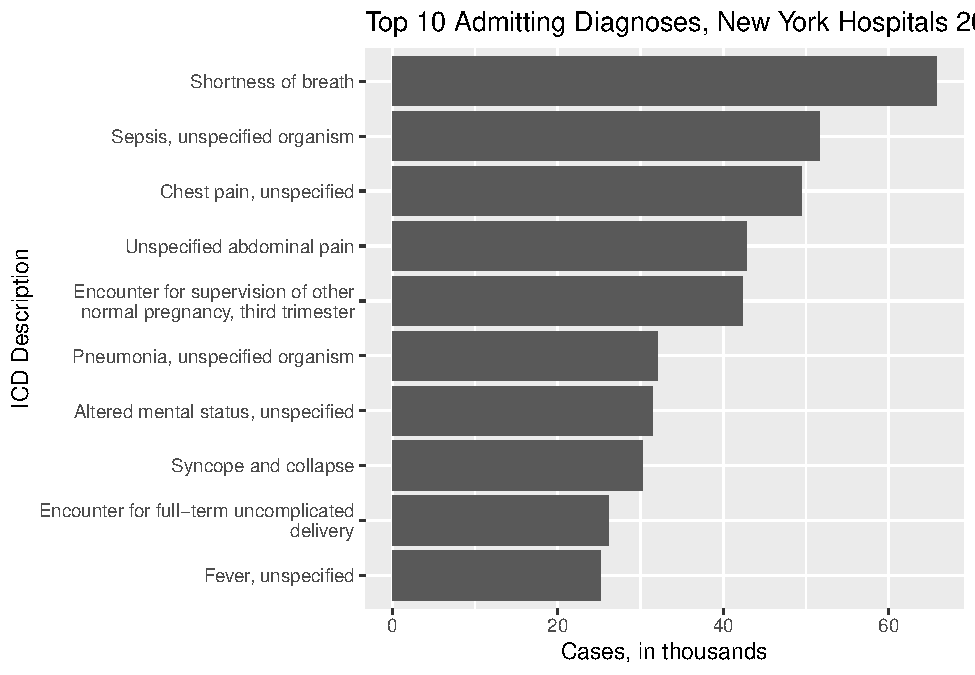
\includegraphics{final-project-paper_files/figure-latex/dx-admitting-1.pdf}

\hypertarget{total-number-of-diagnoses}{%
\paragraph{Total Number of Diagnoses}\label{total-number-of-diagnoses}}

\begin{Shaded}
\begin{Highlighting}[]
\FunctionTok{ggplot}\NormalTok{(ade\_flag, }\FunctionTok{aes}\NormalTok{(I10\_NDX)) }\SpecialCharTok{+} \CommentTok{\#anomaly in the number of diagnoses}
  \FunctionTok{geom\_bar}\NormalTok{() }\SpecialCharTok{+}
    \FunctionTok{scale\_y\_continuous}\NormalTok{(}\AttributeTok{name =} \StringTok{\textquotesingle{}Cases, in thousands\textquotesingle{}}\NormalTok{, }\AttributeTok{labels =} \ControlFlowTok{function}\NormalTok{(y) y }\SpecialCharTok{/}\DecValTok{1000}\NormalTok{) }\SpecialCharTok{+}
  \FunctionTok{labs}\NormalTok{(}\AttributeTok{title=}\StringTok{\textquotesingle{}Anomaly in the Number of Diagnoses\textquotesingle{}}\NormalTok{, }\AttributeTok{x =} \StringTok{\textquotesingle{}Number of ICD{-}10 Diagnoses\textquotesingle{}}\NormalTok{)}
\end{Highlighting}
\end{Shaded}

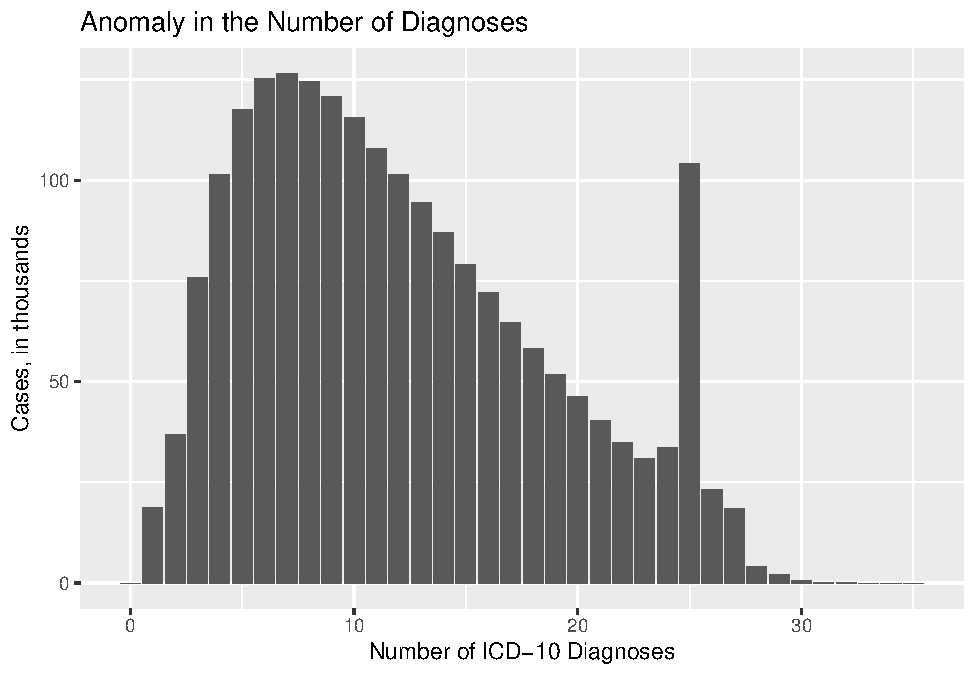
\includegraphics{final-project-paper_files/figure-latex/n-dx-plot-1.pdf}

\hypertarget{most-common-procedures}{%
\subsubsection{Most Common Procedures}\label{most-common-procedures}}

\begin{Shaded}
\begin{Highlighting}[]
\FunctionTok{ggplot}\NormalTok{(ade\_flag, }\FunctionTok{aes}\NormalTok{(I10\_NPR)) }\SpecialCharTok{+}
  \FunctionTok{geom\_bar}\NormalTok{() }\SpecialCharTok{+}
  \FunctionTok{scale\_y\_continuous}\NormalTok{(}\AttributeTok{name =} \StringTok{\textquotesingle{}Cases, in thousands\textquotesingle{}}\NormalTok{, }\AttributeTok{labels =} \ControlFlowTok{function}\NormalTok{(y) y }\SpecialCharTok{/}\DecValTok{1000}\NormalTok{) }\SpecialCharTok{+}
  \FunctionTok{labs}\NormalTok{(}\AttributeTok{title=}\StringTok{\textquotesingle{}Number of ICD{-}10 Procedures\textquotesingle{}}\NormalTok{, }\AttributeTok{x =} \StringTok{\textquotesingle{}Number of ICD{-}10 Diagnoses\textquotesingle{}}\NormalTok{) }
\end{Highlighting}
\end{Shaded}

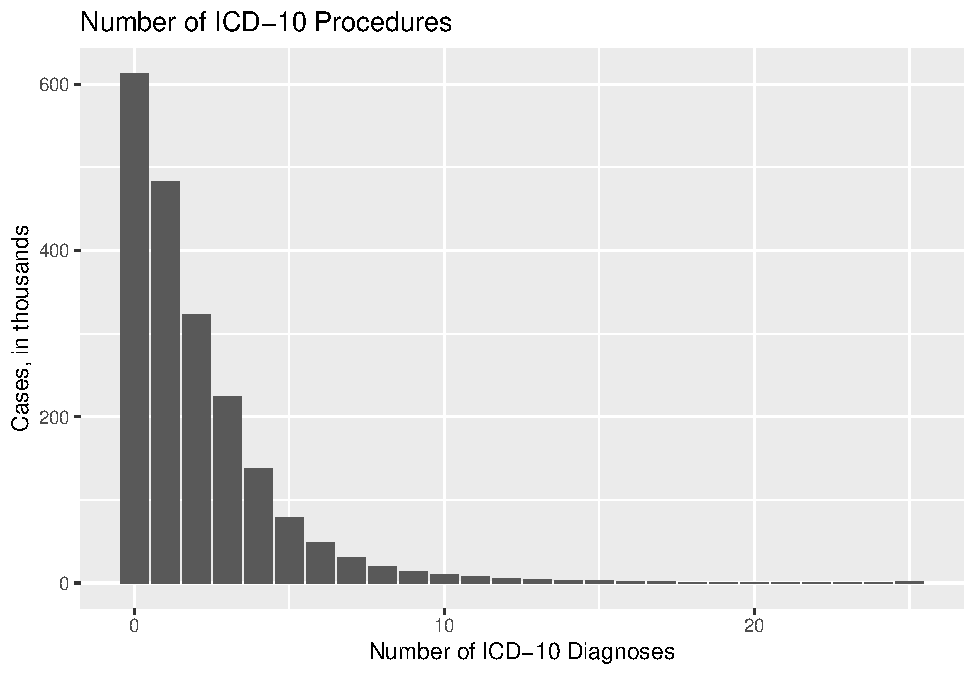
\includegraphics{final-project-paper_files/figure-latex/n-procedures-1.pdf}

\begin{Shaded}
\begin{Highlighting}[]
\NormalTok{i10\_procedure }\OtherTok{\textless{}{-}} \FunctionTok{read.csv}\NormalTok{(}\StringTok{\textquotesingle{}i10\_procedure.csv\textquotesingle{}}\NormalTok{)}


\NormalTok{proc\_counts }\OtherTok{\textless{}{-}}\NormalTok{ ade\_flag }\SpecialCharTok{\%\textgreater{}\%} \CommentTok{\#use similar code to determine most common procedures}
\NormalTok{  dplyr}\SpecialCharTok{::} \FunctionTok{select}\NormalTok{(I10\_PR1}\SpecialCharTok{:}\NormalTok{I10\_PR25) }\SpecialCharTok{\%\textgreater{}\%}
  \FunctionTok{gather}\NormalTok{(dx\_num, Code, I10\_PR1}\SpecialCharTok{:}\NormalTok{I10\_PR25,}\AttributeTok{factor\_key =} \ConstantTok{TRUE}\NormalTok{ ) }\SpecialCharTok{\%\textgreater{}\%}
  \FunctionTok{mutate}\NormalTok{(}\AttributeTok{Code =} \FunctionTok{as.factor}\NormalTok{(Code)) }\SpecialCharTok{\%\textgreater{}\%}
  \FunctionTok{group\_by}\NormalTok{(Code) }\SpecialCharTok{\%\textgreater{}\%}
  \FunctionTok{summarize}\NormalTok{(}\AttributeTok{n\_patients =} \FunctionTok{n}\NormalTok{()) }\SpecialCharTok{\%\textgreater{}\%}
  \FunctionTok{mutate}\NormalTok{(}\AttributeTok{Code =} \FunctionTok{na\_if}\NormalTok{(Code, }\StringTok{\textquotesingle{} \textquotesingle{}}\NormalTok{)) }\SpecialCharTok{\%\textgreater{}\%}
  \FunctionTok{drop\_na}\NormalTok{() }\SpecialCharTok{\%\textgreater{}\%}
  \FunctionTok{arrange}\NormalTok{(}\FunctionTok{desc}\NormalTok{(n\_patients)) }\SpecialCharTok{\%\textgreater{}\%}
  \FunctionTok{inner\_join}\NormalTok{(i10\_procedure, }\AttributeTok{by =} \FunctionTok{c}\NormalTok{(}\StringTok{\textquotesingle{}Code\textquotesingle{}} \OtherTok{=} \StringTok{\textquotesingle{}ICD.10.PCS.CODE\textquotesingle{}}\NormalTok{))  }\SpecialCharTok{\%\textgreater{}\%} \CommentTok{\#join with i10 procedure text csv}
\NormalTok{  dplyr }\SpecialCharTok{::} \FunctionTok{select}\NormalTok{(ICD.}\FloatTok{10.}\NormalTok{PCS.CODE.DESCRIPTION, n\_patients, Code)}


\NormalTok{proc\_counts }\SpecialCharTok{\%\textgreater{}\%}
  \FunctionTok{arrange}\NormalTok{(}\FunctionTok{desc}\NormalTok{(n\_patients)) }\SpecialCharTok{\%\textgreater{}\%}
  \FunctionTok{head}\NormalTok{(}\DecValTok{10}\NormalTok{) }\SpecialCharTok{\%\textgreater{}\%}
  \FunctionTok{ggplot}\NormalTok{(}\FunctionTok{aes}\NormalTok{(}\AttributeTok{x =} \FunctionTok{fct\_reorder}\NormalTok{(ICD.}\FloatTok{10.}\NormalTok{PCS.CODE.DESCRIPTION, n\_patients))) }\SpecialCharTok{+}
  \FunctionTok{geom\_col}\NormalTok{(}\FunctionTok{aes}\NormalTok{(}\AttributeTok{y =}\NormalTok{ n\_patients}\SpecialCharTok{/}\DecValTok{1000}\NormalTok{)) }\SpecialCharTok{+} 
  \FunctionTok{scale\_x\_discrete}\NormalTok{(}\AttributeTok{name =} \StringTok{\textquotesingle{}ICD Description\textquotesingle{}}\NormalTok{, }\AttributeTok{labels =} \ControlFlowTok{function}\NormalTok{(x) }\FunctionTok{str\_wrap}\NormalTok{(}\FunctionTok{str\_replace\_all}\NormalTok{(x, }\StringTok{"foo"}\NormalTok{ , }\StringTok{" "}\NormalTok{), }\AttributeTok{width =} \DecValTok{55}\NormalTok{)) }\SpecialCharTok{+}
  \FunctionTok{theme}\NormalTok{(}\AttributeTok{legend.position =} \FunctionTok{c}\NormalTok{(}\FloatTok{0.75}\NormalTok{,}\FloatTok{0.25}\NormalTok{)) }\SpecialCharTok{+}
  \FunctionTok{labs}\NormalTok{(}\AttributeTok{title =} \StringTok{\textquotesingle{}Top 10 Most Common Procedures\textquotesingle{}}\NormalTok{) }\SpecialCharTok{+}
  \FunctionTok{scale\_y\_continuous}\NormalTok{(}\AttributeTok{name =} \StringTok{\textquotesingle{}ICD{-}10 Procedure Claims, in thousands\textquotesingle{}}\NormalTok{) }\SpecialCharTok{+}
  \FunctionTok{coord\_flip}\NormalTok{() }
\end{Highlighting}
\end{Shaded}

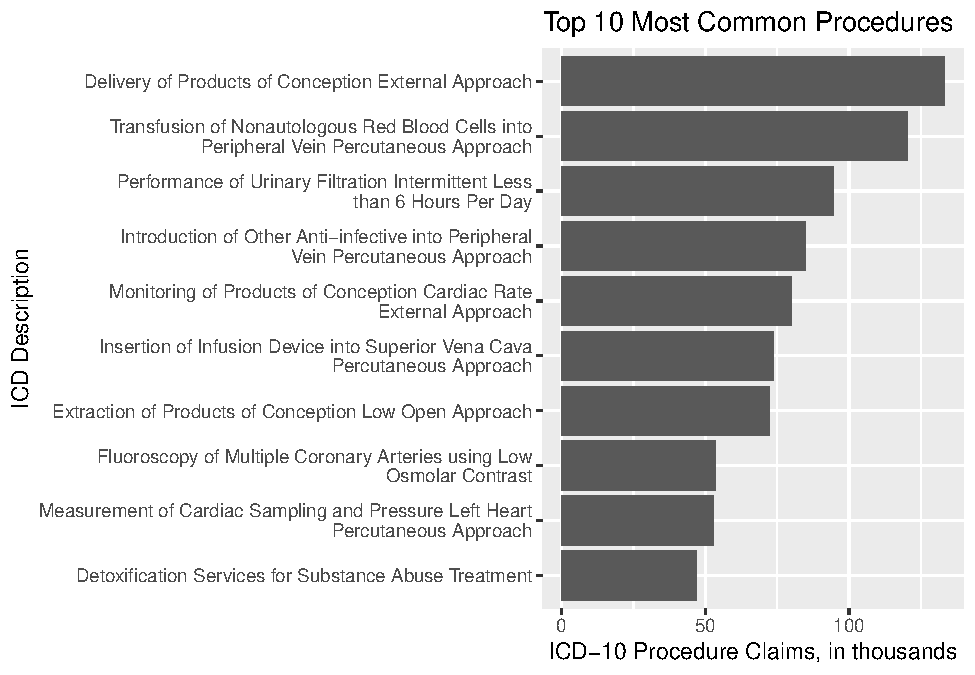
\includegraphics{final-project-paper_files/figure-latex/top-10-procedures-1.pdf}

\hypertarget{top-adverse-drug-events}{%
\subsubsection{Top Adverse Drug Events}\label{top-adverse-drug-events}}

\begin{Shaded}
\begin{Highlighting}[]
\FunctionTok{rm}\NormalTok{(ade\_cost)}


\NormalTok{ade\_counts }\OtherTok{\textless{}{-}}\NormalTok{ ade\_flag }\SpecialCharTok{\%\textgreater{}\%}
  \FunctionTok{filter}\NormalTok{(has\_ade }\SpecialCharTok{==} \DecValTok{1}\NormalTok{) }\SpecialCharTok{\%\textgreater{}\%}
  \FunctionTok{group\_by}\NormalTok{(Code, Description) }\SpecialCharTok{\%\textgreater{}\%}
  \FunctionTok{summarize}\NormalTok{(}\AttributeTok{n\_icd =} \FunctionTok{n}\NormalTok{()) }\SpecialCharTok{\%\textgreater{}\%}
  \FunctionTok{left\_join}\NormalTok{(icd, }\FunctionTok{c}\NormalTok{(}\StringTok{\textquotesingle{}Code\textquotesingle{}} \OtherTok{=} \StringTok{\textquotesingle{}V3\textquotesingle{}}\NormalTok{)) }\SpecialCharTok{\%\textgreater{}\%}
  \FunctionTok{arrange}\NormalTok{(}\FunctionTok{desc}\NormalTok{(n\_icd)) }\SpecialCharTok{\%\textgreater{}\%}
  \FunctionTok{mutate}\NormalTok{(}\AttributeTok{Description =} \FunctionTok{fct\_relevel}\NormalTok{(Description, }\FunctionTok{c}\NormalTok{(}\StringTok{\textquotesingle{}Category A1\textquotesingle{}}\NormalTok{,}\StringTok{\textquotesingle{}Category A2\textquotesingle{}}\NormalTok{, }\StringTok{\textquotesingle{}Category B2\textquotesingle{}}\NormalTok{, }\StringTok{\textquotesingle{}Category C\textquotesingle{}}\NormalTok{)))}
\end{Highlighting}
\end{Shaded}

\begin{verbatim}
## `summarise()` has grouped output by 'Code'. You can override using the
## `.groups` argument.
\end{verbatim}

\begin{Shaded}
\begin{Highlighting}[]
\NormalTok{ade\_counts }\SpecialCharTok{\%\textgreater{}\%}
  \FunctionTok{head}\NormalTok{(}\DecValTok{10}\NormalTok{) }\SpecialCharTok{\%\textgreater{}\%}
  \FunctionTok{ggplot}\NormalTok{(}\FunctionTok{aes}\NormalTok{(}\AttributeTok{x =} \FunctionTok{fct\_reorder}\NormalTok{(V5, n\_icd))) }\SpecialCharTok{+}
  \FunctionTok{geom\_col}\NormalTok{(}\FunctionTok{aes}\NormalTok{(}\AttributeTok{y =}\NormalTok{ n\_icd}\SpecialCharTok{/}\DecValTok{1000}\NormalTok{, }\AttributeTok{fill =}\NormalTok{ Description)) }\SpecialCharTok{+} 
  \FunctionTok{scale\_x\_discrete}\NormalTok{(}\AttributeTok{name =} \StringTok{\textquotesingle{}ICD Description\textquotesingle{}}\NormalTok{, }\AttributeTok{labels =} \ControlFlowTok{function}\NormalTok{(x) }\FunctionTok{str\_wrap}\NormalTok{(}\FunctionTok{str\_replace\_all}\NormalTok{(x, }\StringTok{"foo"}\NormalTok{ , }\StringTok{" "}\NormalTok{),}
                                                 \AttributeTok{width =} \DecValTok{40}\NormalTok{)) }\SpecialCharTok{+}
  \FunctionTok{theme}\NormalTok{(}\AttributeTok{legend.position =} \FunctionTok{c}\NormalTok{(}\FloatTok{0.75}\NormalTok{,}\FloatTok{0.25}\NormalTok{)) }\SpecialCharTok{+}
  \FunctionTok{labs}\NormalTok{(}\AttributeTok{title =} \StringTok{\textquotesingle{}Top 10 Most Common ADE}\SpecialCharTok{\textbackslash{}\textquotesingle{}}\StringTok{s, 2018\textquotesingle{}}\NormalTok{) }\SpecialCharTok{+}
  \FunctionTok{scale\_y\_continuous}\NormalTok{(}\AttributeTok{name =} \StringTok{\textquotesingle{}Cases, in thousands\textquotesingle{}}\NormalTok{) }\SpecialCharTok{+}
  \FunctionTok{coord\_flip}\NormalTok{() }
\end{Highlighting}
\end{Shaded}

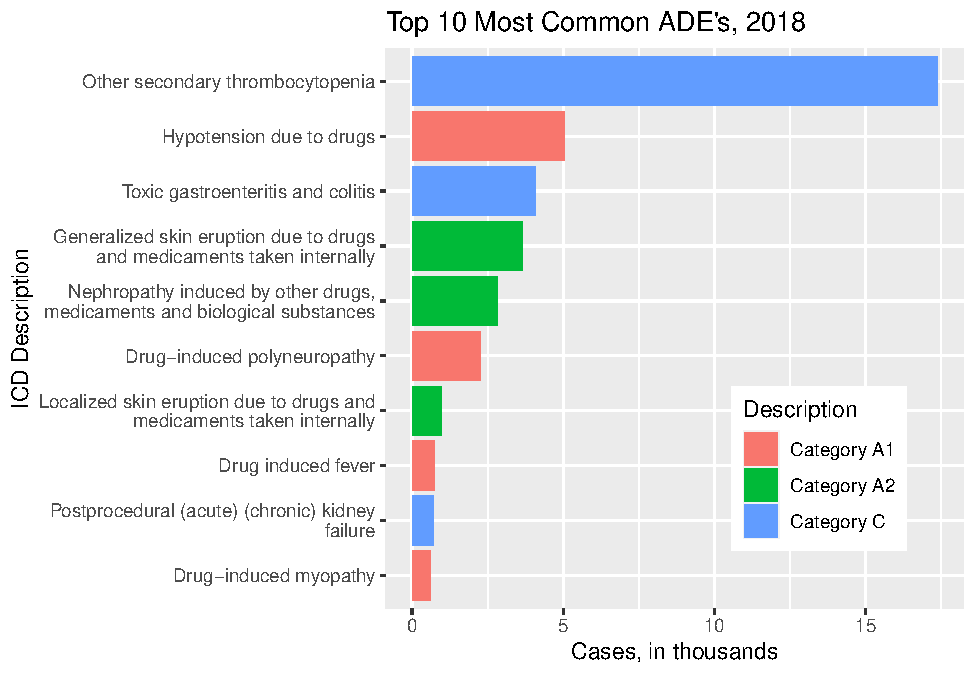
\includegraphics{final-project-paper_files/figure-latex/top-10-ade-1.pdf}

\begin{Shaded}
\begin{Highlighting}[]
\NormalTok{ade\_counts2 }\OtherTok{\textless{}{-}}\NormalTok{ ade\_flag }\SpecialCharTok{\%\textgreater{}\%}
  \FunctionTok{filter}\NormalTok{(has\_ade }\SpecialCharTok{==} \DecValTok{1}\NormalTok{) }\SpecialCharTok{\%\textgreater{}\%}
  \FunctionTok{filter}\NormalTok{(Description }\SpecialCharTok{!=} \StringTok{\textquotesingle{}Category C\textquotesingle{}}\NormalTok{) }\SpecialCharTok{\%\textgreater{}\%}
  \FunctionTok{group\_by}\NormalTok{(Code, Description) }\SpecialCharTok{\%\textgreater{}\%}
  \FunctionTok{summarize}\NormalTok{(}\AttributeTok{n\_icd =} \FunctionTok{n}\NormalTok{()) }\SpecialCharTok{\%\textgreater{}\%}
  \FunctionTok{left\_join}\NormalTok{(icd, }\FunctionTok{c}\NormalTok{(}\StringTok{\textquotesingle{}Code\textquotesingle{}} \OtherTok{=} \StringTok{\textquotesingle{}V3\textquotesingle{}}\NormalTok{)) }\SpecialCharTok{\%\textgreater{}\%}
  \FunctionTok{arrange}\NormalTok{(}\FunctionTok{desc}\NormalTok{(n\_icd)) }\SpecialCharTok{\%\textgreater{}\%}
  \FunctionTok{mutate}\NormalTok{(}\AttributeTok{Description =} \FunctionTok{fct\_relevel}\NormalTok{(Description, }\FunctionTok{c}\NormalTok{(}\StringTok{\textquotesingle{}Category A1\textquotesingle{}}\NormalTok{,}\StringTok{\textquotesingle{}Category A2\textquotesingle{}}\NormalTok{, }\StringTok{\textquotesingle{}Category B2\textquotesingle{}}\NormalTok{, }\StringTok{\textquotesingle{}Category C\textquotesingle{}}\NormalTok{)))}
\end{Highlighting}
\end{Shaded}

\begin{verbatim}
## `summarise()` has grouped output by 'Code'. You can override using the
## `.groups` argument.
\end{verbatim}

\begin{Shaded}
\begin{Highlighting}[]
\NormalTok{ade\_counts2 }\SpecialCharTok{\%\textgreater{}\%}
  \FunctionTok{head}\NormalTok{(}\DecValTok{10}\NormalTok{) }\SpecialCharTok{\%\textgreater{}\%}
  \FunctionTok{ggplot}\NormalTok{(}\FunctionTok{aes}\NormalTok{(}\AttributeTok{x =} \FunctionTok{fct\_reorder}\NormalTok{(V5, n\_icd))) }\SpecialCharTok{+}
  \FunctionTok{geom\_col}\NormalTok{(}\FunctionTok{aes}\NormalTok{(}\AttributeTok{y =}\NormalTok{ n\_icd}\SpecialCharTok{/}\DecValTok{1000}\NormalTok{, }\AttributeTok{fill =}\NormalTok{ Description)) }\SpecialCharTok{+} 
  \FunctionTok{scale\_x\_discrete}\NormalTok{(}\AttributeTok{name =} \StringTok{\textquotesingle{}ICD Description\textquotesingle{}}\NormalTok{, }\AttributeTok{labels =} \ControlFlowTok{function}\NormalTok{(x) }\FunctionTok{str\_wrap}\NormalTok{(}\FunctionTok{str\_replace\_all}\NormalTok{(x, }\StringTok{"foo"}\NormalTok{ , }\StringTok{" "}\NormalTok{),}
                                                 \AttributeTok{width =} \DecValTok{40}\NormalTok{)) }\SpecialCharTok{+}
  \FunctionTok{theme}\NormalTok{(}\AttributeTok{legend.position =} \FunctionTok{c}\NormalTok{(}\FloatTok{0.75}\NormalTok{,}\FloatTok{0.25}\NormalTok{)) }\SpecialCharTok{+}
  \FunctionTok{labs}\NormalTok{(}\AttributeTok{title =} \StringTok{\textquotesingle{}Most Common Category }\SpecialCharTok{\textbackslash{}\textquotesingle{}}\StringTok{A}\SpecialCharTok{\textbackslash{}\textquotesingle{}}\StringTok{ drug reactions\textquotesingle{}}\NormalTok{) }\SpecialCharTok{+}
  \FunctionTok{scale\_y\_continuous}\NormalTok{(}\AttributeTok{name =} \StringTok{\textquotesingle{}Cases, in thousands\textquotesingle{}}\NormalTok{) }\SpecialCharTok{+}
  \FunctionTok{coord\_flip}\NormalTok{() }
\end{Highlighting}
\end{Shaded}

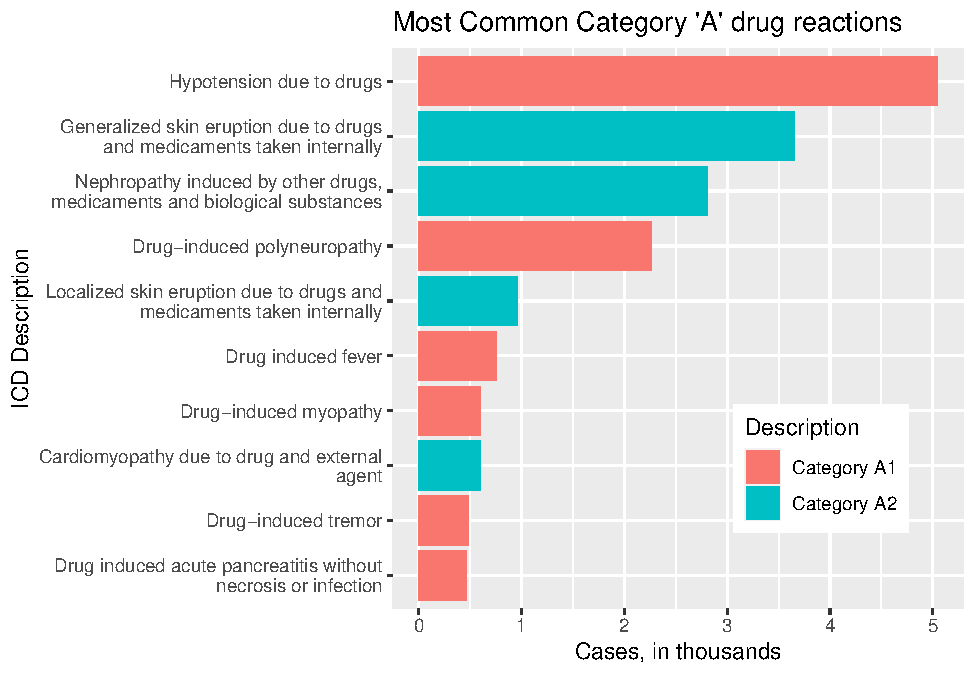
\includegraphics{final-project-paper_files/figure-latex/top-10-ade-cat-a-1.pdf}

\begin{Shaded}
\begin{Highlighting}[]
\NormalTok{ade\_counts2 }\SpecialCharTok{\%\textgreater{}\%}
  \FunctionTok{filter}\NormalTok{(Description }\SpecialCharTok{==} \StringTok{\textquotesingle{}Category B2\textquotesingle{}}\NormalTok{) }\SpecialCharTok{\%\textgreater{}\%}
  \FunctionTok{head}\NormalTok{(}\DecValTok{10}\NormalTok{) }\SpecialCharTok{\%\textgreater{}\%}
  \FunctionTok{ggplot}\NormalTok{(}\FunctionTok{aes}\NormalTok{(}\AttributeTok{x =} \FunctionTok{fct\_reorder}\NormalTok{(V5, n\_icd))) }\SpecialCharTok{+}
  \FunctionTok{geom\_col}\NormalTok{(}\FunctionTok{aes}\NormalTok{(}\AttributeTok{y =}\NormalTok{ n\_icd)) }\SpecialCharTok{+} 
  \FunctionTok{scale\_x\_discrete}\NormalTok{(}\AttributeTok{name =} \StringTok{\textquotesingle{}ICD Description\textquotesingle{}}\NormalTok{, }\AttributeTok{labels =} \ControlFlowTok{function}\NormalTok{(x) }\FunctionTok{str\_wrap}\NormalTok{(}\FunctionTok{str\_replace\_all}\NormalTok{(x, }\StringTok{"foo"}\NormalTok{ , }\StringTok{" "}\NormalTok{),}
                                                 \AttributeTok{width =} \DecValTok{35}\NormalTok{)) }\SpecialCharTok{+}
  \FunctionTok{labs}\NormalTok{(}\AttributeTok{title =} \StringTok{\textquotesingle{}Most Common Category }\SpecialCharTok{\textbackslash{}\textquotesingle{}}\StringTok{B}\SpecialCharTok{\textbackslash{}\textquotesingle{}}\StringTok{ drug reactions\textquotesingle{}}\NormalTok{) }\SpecialCharTok{+}
  \FunctionTok{scale\_y\_continuous}\NormalTok{(}\AttributeTok{name =} \StringTok{\textquotesingle{}Cases\textquotesingle{}}\NormalTok{) }\SpecialCharTok{+}
  \FunctionTok{coord\_flip}\NormalTok{() }
\end{Highlighting}
\end{Shaded}

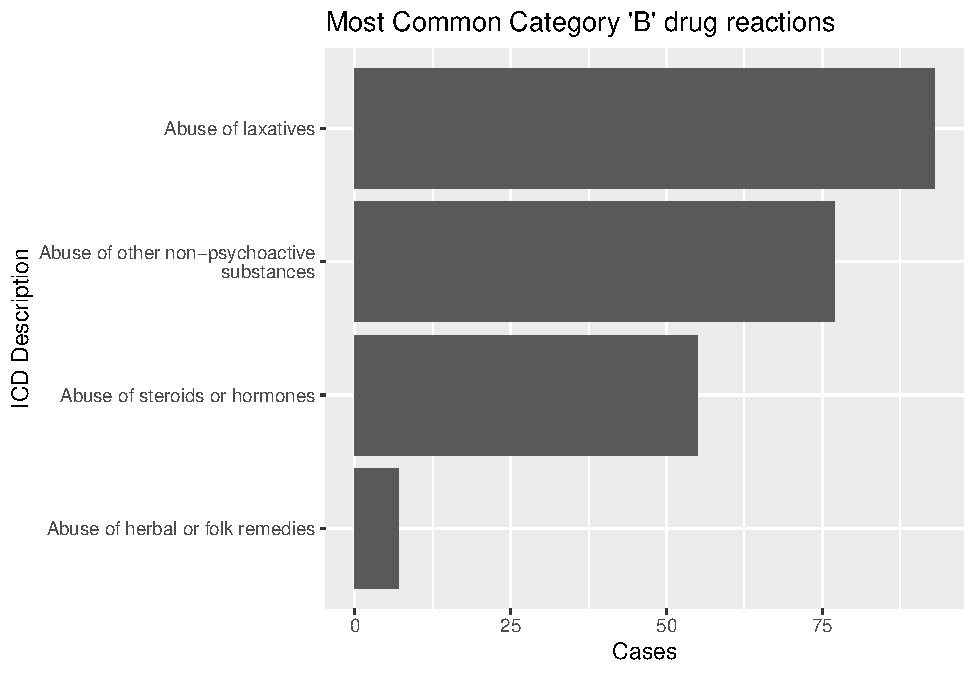
\includegraphics{final-project-paper_files/figure-latex/ade-cat-B-1.pdf}

\begin{Shaded}
\begin{Highlighting}[]
\NormalTok{ade\_counts }\SpecialCharTok{\%\textgreater{}\%}
  \FunctionTok{filter}\NormalTok{(Description }\SpecialCharTok{==} \StringTok{\textquotesingle{}Category C\textquotesingle{}}\NormalTok{) }\SpecialCharTok{\%\textgreater{}\%}
  \FunctionTok{head}\NormalTok{(}\DecValTok{3}\NormalTok{) }\SpecialCharTok{\%\textgreater{}\%}
  \FunctionTok{ggplot}\NormalTok{(}\FunctionTok{aes}\NormalTok{(}\AttributeTok{x =} \FunctionTok{fct\_reorder}\NormalTok{(V5, n\_icd))) }\SpecialCharTok{+}
  \FunctionTok{geom\_col}\NormalTok{(}\FunctionTok{aes}\NormalTok{(}\AttributeTok{y =}\NormalTok{ n\_icd}\SpecialCharTok{/}\DecValTok{1000}\NormalTok{)) }\SpecialCharTok{+} 
  \FunctionTok{scale\_x\_discrete}\NormalTok{(}\AttributeTok{name =} \StringTok{\textquotesingle{}ICD Description\textquotesingle{}}\NormalTok{, }\AttributeTok{labels =} \ControlFlowTok{function}\NormalTok{(x) }\FunctionTok{str\_wrap}\NormalTok{(}\FunctionTok{str\_replace\_all}\NormalTok{(x, }\StringTok{"foo"}\NormalTok{ , }\StringTok{" "}\NormalTok{),}
                                                 \AttributeTok{width =} \DecValTok{35}\NormalTok{)) }\SpecialCharTok{+}
  \FunctionTok{labs}\NormalTok{(}\AttributeTok{title =} \StringTok{\textquotesingle{}Most Common Category }\SpecialCharTok{\textbackslash{}\textquotesingle{}}\StringTok{C}\SpecialCharTok{\textbackslash{}\textquotesingle{}}\StringTok{ drug reactions\textquotesingle{}}\NormalTok{) }\SpecialCharTok{+}
  \FunctionTok{scale\_y\_continuous}\NormalTok{(}\AttributeTok{name =} \StringTok{\textquotesingle{}Cases, in thousands\textquotesingle{}}\NormalTok{) }\SpecialCharTok{+}
  \FunctionTok{coord\_flip}\NormalTok{() }
\end{Highlighting}
\end{Shaded}

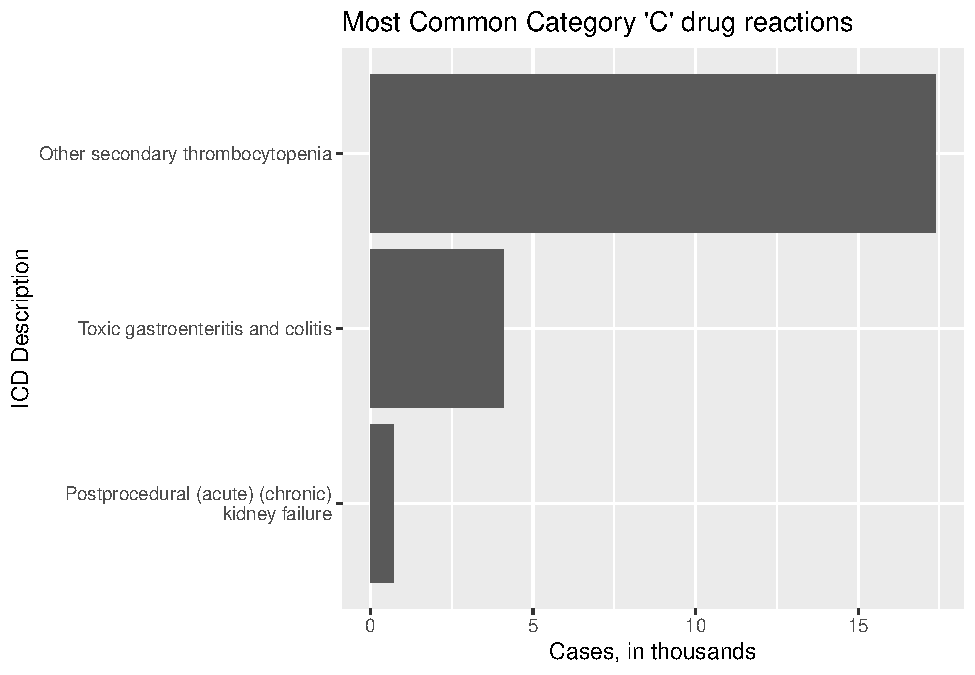
\includegraphics{final-project-paper_files/figure-latex/ade-cat-c-1.pdf}

\hypertarget{target-prediction}{%
\subsubsection{Target Prediction}\label{target-prediction}}

\hypertarget{techniques}{%
\paragraph{Techniques}\label{techniques}}

\hypertarget{model-performance}{%
\paragraph{Model Performance}\label{model-performance}}

\begin{Shaded}
\begin{Highlighting}[]
\NormalTok{performance\_df }\OtherTok{\textless{}{-}} \FunctionTok{read.csv}\NormalTok{(}\StringTok{\textquotesingle{}models\_performance.csv\textquotesingle{}}\NormalTok{)}

\NormalTok{performance\_df }\OtherTok{\textless{}{-}}\NormalTok{ performance\_df }\SpecialCharTok{\%\textgreater{}\%}
  \FunctionTok{mutate}\NormalTok{(}\AttributeTok{Accuracy =} \DecValTok{100}\SpecialCharTok{*}\FunctionTok{round}\NormalTok{((TP}\SpecialCharTok{+}\NormalTok{TN)}\SpecialCharTok{/}\NormalTok{(TP}\SpecialCharTok{+}\NormalTok{TN}\SpecialCharTok{+}\NormalTok{FP}\SpecialCharTok{+}\NormalTok{FN),}\DecValTok{3}\NormalTok{)) }\SpecialCharTok{\%\textgreater{}\%}
  \FunctionTok{mutate}\NormalTok{(}\AttributeTok{Precision =} \DecValTok{100}\SpecialCharTok{*}\FunctionTok{round}\NormalTok{(TP}\SpecialCharTok{/}\NormalTok{(TP }\SpecialCharTok{+}\NormalTok{ FP),}\DecValTok{3}\NormalTok{)) }\SpecialCharTok{\%\textgreater{}\%}
  \FunctionTok{mutate}\NormalTok{(}\AttributeTok{Recall =} \DecValTok{100}\SpecialCharTok{*}\FunctionTok{round}\NormalTok{(TP}\SpecialCharTok{/}\NormalTok{(TP }\SpecialCharTok{+}\NormalTok{ FN),}\DecValTok{3}\NormalTok{))}

\NormalTok{performance\_df }\OtherTok{\textless{}{-}}\NormalTok{ performance\_df }\SpecialCharTok{\%\textgreater{}\%}
  \FunctionTok{mutate}\NormalTok{(}\AttributeTok{F1 =} \FunctionTok{round}\NormalTok{(}\DecValTok{2}\SpecialCharTok{*}\NormalTok{Precision}\SpecialCharTok{*}\NormalTok{Recall}\SpecialCharTok{/}\NormalTok{(Precision }\SpecialCharTok{+}\NormalTok{ Recall)}\SpecialCharTok{/}\DecValTok{100}\NormalTok{,}\DecValTok{2}\NormalTok{)) }\SpecialCharTok{\%\textgreater{}\%}
  \FunctionTok{mutate}\NormalTok{(}\AttributeTok{TPR =} \DecValTok{100}\SpecialCharTok{*}\FunctionTok{round}\NormalTok{(TP}\SpecialCharTok{/}\NormalTok{(TP}\SpecialCharTok{+}\NormalTok{FN),}\DecValTok{3}\NormalTok{)) }\SpecialCharTok{\%\textgreater{}\%}
  \FunctionTok{select}\NormalTok{(}\SpecialCharTok{{-}}\NormalTok{TN,}\SpecialCharTok{{-}}\NormalTok{TP,}\SpecialCharTok{{-}}\NormalTok{FN,}\SpecialCharTok{{-}}\NormalTok{FP)}


\NormalTok{performance\_df }\SpecialCharTok{\%\textgreater{}\%}
  \FunctionTok{gt}\NormalTok{() }\SpecialCharTok{\%\textgreater{}\%}
  \FunctionTok{tab\_header}\NormalTok{(}\StringTok{"Selected Model Performance for the Detection of Adverse Drug Events"}\NormalTok{)}
\end{Highlighting}
\end{Shaded}

\captionsetup[table]{labelformat=empty,skip=1pt}
\begin{longtable}{lrrrrr}
\caption*{
{\large Selected Model Performance for the Detection of Adverse Drug Events}
} \\ 
\toprule
Model & Accuracy & Precision & Recall & F1 & TPR \\ 
\midrule
GLM & 77.6 & 6.7 & 71.9 & 0.12 & 71.9 \\ 
SGB & 77.2 & 7.4 & 82.4 & 0.14 & 82.4 \\ 
Random Forest & 2.2 & 5.6 & 2.2 & 0.03 & 2.2 \\ 
Neural Net & 67.9 & 5.6 & 85.6 & 0.11 & 85.6 \\ 
\bottomrule
\end{longtable}

\hypertarget{conclusions-and-future-directions}{%
\subsection{Conclusions and Future
Directions}\label{conclusions-and-future-directions}}

\bibliography{mybibfile.bib}


\end{document}
